%%%%%%%%%%%%%%%%%%%%%%%%%%%%%%%%%%%%%%%%%
% Thin Sectioned Essay
% LaTeX Template
% Version 1.0 (3/8/13)
%
% This template has been downloaded from:
% http://www.LaTeXTemplates.com
%
% Original Author:
% Nicolas Diaz (nsdiaz@uc.cl) with extensive modifications by:
% Vel (vel@latextemplates.com)
%
% License:
% CC BY-NC-SA 3.0 (http://creativecommons.org/licenses/by-nc-sa/3.0/)
%
%%%%%%%%%%%%%%%%%%%%%%%%%%%%%%%%%%%%%%%%%

%----------------------------------------------------------------------------------------
%	PACKAGES AND OTHER DOCUMENT CONFIGURATIONS
%----------------------------------------------------------------------------------------

\documentclass[a4paper, 11pt]{article} % Font size (can be 10pt, 11pt or 12pt) and paper size (remove a4paper for US letter paper)

\usepackage[protrusion=true,expansion=true]{microtype} % Better typography
\usepackage{graphicx} % Required for including pictures
%\usepackage[font=small]{subfig}
\graphicspath{{images/}}
\DeclareGraphicsExtensions{.pdf,.png,.jpg}

\usepackage{wrapfig} % Allows in-line images

\usepackage{mathpazo} % Use the Palatino font
\usepackage[T1]{fontenc} % Required for accented characters
\linespread{1.05} % Change line spacing here, Palatino benefits from a slight increase by default

\makeatletter
\renewcommand\@biblabel[1]{\textbf{#1.}} % Change the square brackets for each bibliography item from '[1]' to '1.'
\renewcommand{\@listI}{\itemsep=0pt} % Reduce the space between items in the itemize and enumerate environments and the bibliography

\renewcommand{\maketitle}{ % Customize the title - do not edit title and author name here, see the TITLE block below
\begin{flushright} % Right align
{\LARGE\@title} % Increase the font size of the title

\vspace{50pt} % Some vertical space between the title and author name

{\large\@author} % Author name
\\\@date % Date

\vspace{40pt} % Some vertical space between the author block and abstract
\end{flushright}
}

%----------------------------------------------------------------------------------------
%	TITLE
%----------------------------------------------------------------------------------------

\title{\textbf{Electrical Generator Technologies for Offshore Wind Turbines}} % Subtitle

\author{\textsc{Ozan Keysan} % Author
\\{\textit{Institute for Energy  Systems\\ University of Edinburgh}}} % Institution

\date{\today} % Date

%----------------------------------------------------------------------------------------

\begin{document}

\maketitle % Print the title section

%----------------------------------------------------------------------------------------
%	ABSTRACT AND KEYWORDS
%----------------------------------------------------------------------------------------

%\renewcommand{\abstractname}{Summary} % Uncomment to change the name of the abstract to something else

\begin{abstract}

Different electric generator options for offshore wind turbines will be reviewed in this chapter.

Morbi tempor congue porta. Proin semper, leo vitae faucibus dictum, metus mauris lacinia lorem, ac congue leo felis eu turpis. Sed nec nunc pellentesque, gravida eros at, porttitor ipsum. Praesent consequat urna a lacus lobortis ultrices eget ac metus. In tempus hendrerit rhoncus. Mauris dignissim turpis id sollicitudin lacinia. Praesent libero tellus, fringilla nec ullamcorper at, ultrices id nulla. Phasellus placerat a tellus a malesuada.
\end{abstract}

\hspace*{3,6mm}\textit{Keywords:} lorem , ipsum , dolor , sit amet , lectus % Keywords

\vspace{30pt} % Some vertical space between the abstract and first section

%----------------------------------------------------------------------------------------
%	ESSAY BODY
%----------------------------------------------------------------------------------------

\section*{Introduction}


The mechanical energy captured by the turbine blades are converted to electrical energy and is fed into the grid with a series of components such as; gearbox, generator, power electronics, transformer and transmission. Generator is the most important component in the power take-off system and there are many different types of generator types that can be used in turbines depending on the size, operating conditions, and speed range. Some generator types used in commercial wind turbines are presented in Table \ref{generator_manufacturers}. In this chapter,  the generators presented in the table as well as the a few other novel generator concepts will be investigated.


%GE machine specs
\begin{table}[t]
  \centering
  \begin{tabular}{clrrlc}
	  
	  Drive Train & Generator & Power & Rotor & Rated & Manufacturer \\
	  \hline
		& DFIG & 2 MW & 90 m & 20.7 rpm & DeWind \\
		& DFIG & 2 MW & 90 m & 19 rpm & Gamesa \\
	  	& WRIG & 2 MW & 88 m &  & Suzlon \\
	  	& PMSG & 2 MW & 88 m & 16.5 rpm & General Electric \\
	 Multiple 	& DFIG & 2.5 MW & 90 m & 14.9 rpm & Nordex \\
	Stage  	& DFIG & 3 MW & 100 m & 14.3 rpm & Ecotecnia \\
  	Gearbox & DFIG & 3.6 MW & 104 m & 15.3 rpm & General Electric \\
	  	& DFIG & 4.5 MW & 120 m & 14.9 rpm & Vestas \\
	  	& DFIG & 6 MW & 126 m & 12.1 rpm & RePower \\
	  	\hline
	Single--Stage  	& PMSG & 3 MW & 90 m & 18 rpm & Winwind \\
	Gearbox  	& PMSG & 5 MW & 116 m & 14.8 rpm & Multibrid \\
	  	\hline
	 Hydraulic 	& EESG & 2 MW & 90 m & 20.7 rpm & DeWind \\
	 Transmission 	& EESG & 2.4 MW &  & 10 rpm & Mitsubishi \\
	  	\hline
	  	& PMSG & 1.5 MW & 77 m & 17.3 rpm & Vensys \\
	  	& EESG & 1.6 MW & 78 m &  & MTOI \\
	  	& PMSG & 2 MW &  &  & Mitsubishi \\
	Direct-Drive  	& PMSG & 2 MW & 71 m & 23 rpm & Zephyros \\
	  	& PMSG & 3 MW & 101 m & 14.4 rpm & LeitWind \\
	  	& EESG & 4.5 MW & 114 m & 13 rpm & Enercon \\
	  	& EESG & 7.5 MW & 127 m & 11.7 rpm & Enercon \\
	  \hline

  \end{tabular}
  \caption{Drive train types of some commercial wind turbines \cite{wind_energy_facts,upwind2011}.}
  \label{generator_manufacturers}
\end{table}

\section{Doubly-fed Induction Generator}

Doubly-fed induction generator coupled with three-stage gearbox (DFIG-3G) is the most common power take-off system in wind turbines, with more than half of the market share. Some of the wind turbine companies that use this configuration have been presented in Table \ref{generator_manufacturers}.
In Figure \ref{repower} one of the largest DFIG wind turbines(6~MW) are presented, which are  manufactured by RePower.
DFIG generators are usually coupled with multi-stage gearboxes to increase the rotational speed. DFIGs rotational speed is close to the synchronous speed (e.g. 1500~rpm for a 4-pole machine in a 50~Hz grid).

  \begin{figure}
    \centering
    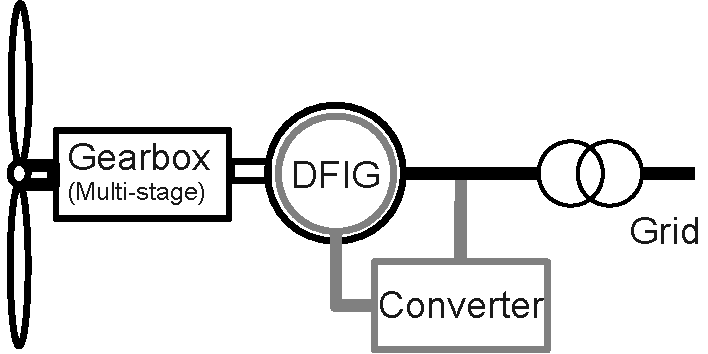
\includegraphics[width=0.5\textwidth]{DFIG_3G}
    \caption{Doubly-fed induction generator coupled to multi-stage gearbox.} 
    \label{dfig_3g}
  \end{figure}

Doubly-fed induction generator is a special type of induction machine. DFIGs differ from squirrel-cage induction generators as they need wound-rotor and electrical brushes. The frequency of the armature voltage is controlled by the field winding. Armature winding of the doubly-fed induction generator is directly connected to the grid. Therefore, DFIGs do not require full-rating power electronics, which is the main advantage of this generator type. The rating of the converter is about 25--30\% of the generator capacity, which reduces the overall cost \cite{Li2008a} . 

The advantages of the DFIG system can be listed as;

\begin{itemize}
	\item Partially rated power electronics reduces the cost.
	\item Ability to supply reactive power to the grid.
	\item Off-the-shelf components, wide range of generator options.
\end{itemize}

However, DFIGs also have a few disadvantages \cite{Li2008a}:

\begin{itemize}
	\item A multi-stage gearbox is necessary which may cause reliability issues.
	\item A slip ring is used, which require regular maintenance.
	\item High torque peaks in the machine and large stator peak currents under grid fault conditions. The power electronics should be protected.
	\item In case of grid disturbances, the ride-through requirements make the DFIG control complex.
\end{itemize}

\begin{figure}[]
  \centering
  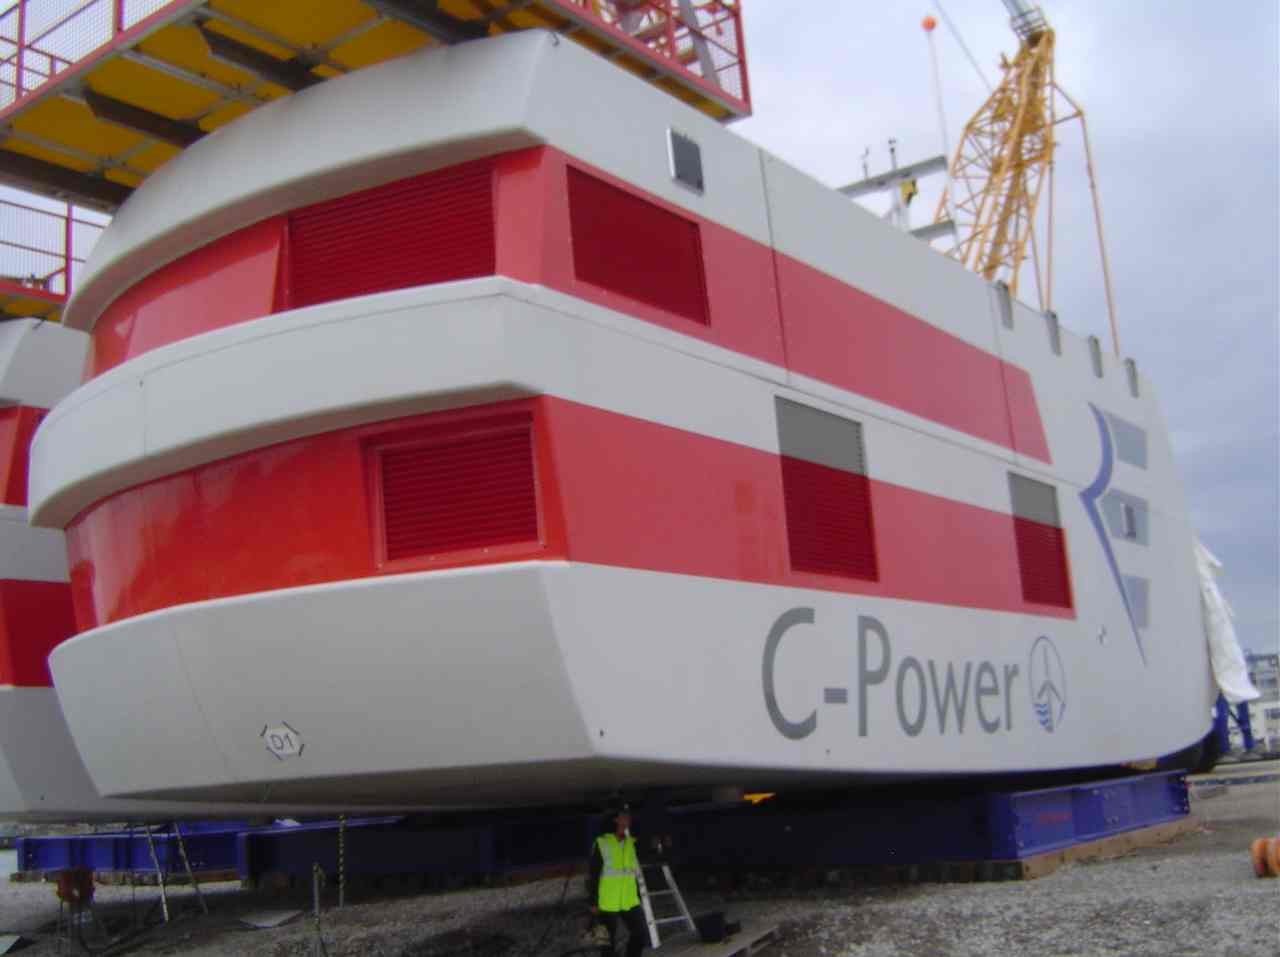
\includegraphics[width=0.45\textwidth]{repower_nacelle}
  \hfill
    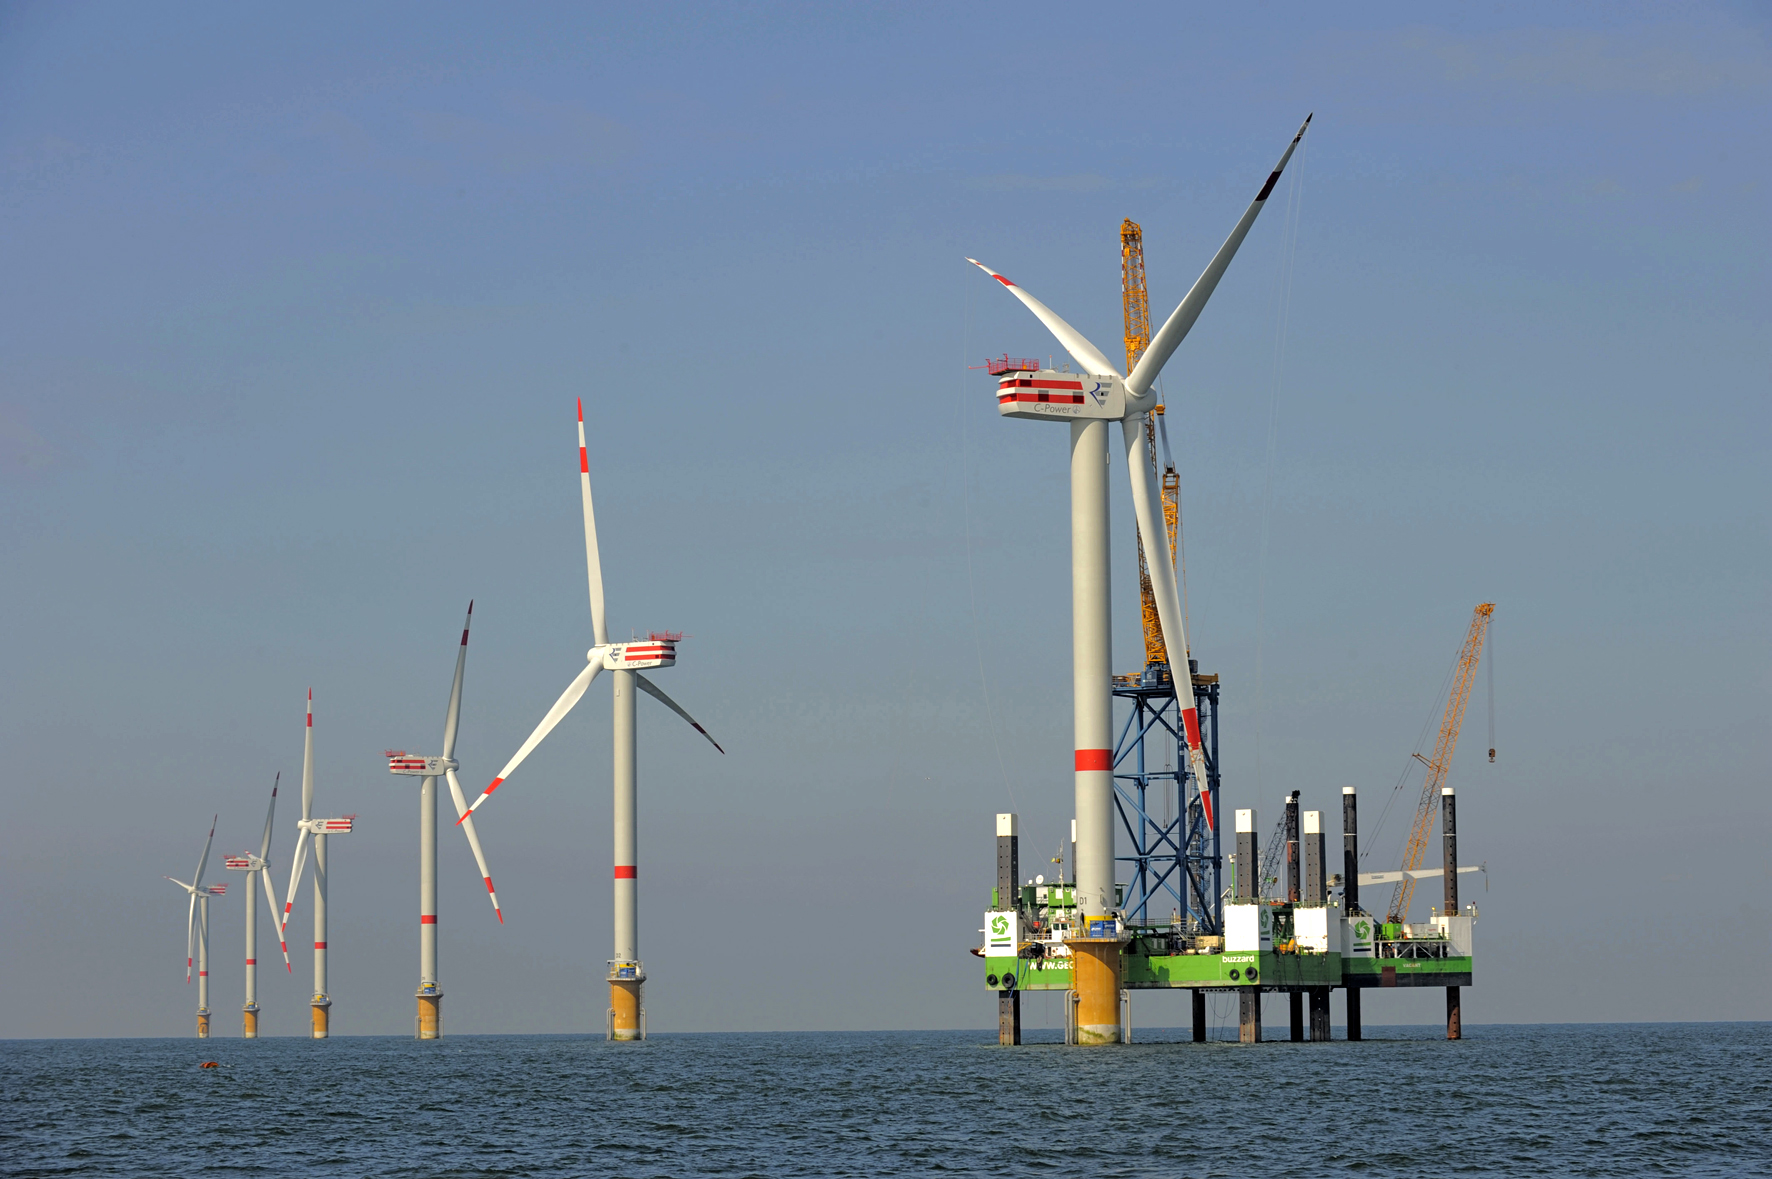
\includegraphics[width=0.5\textwidth]{repower_farm}
\caption{RePower 6 MW wind turbines with DFIG (Courtesy of RePower, Jerome a Paris).}
  \label{repower}
\end{figure}

\section{Direct Drive}

In direct-drive systems, the generator is directly connected to the turbine, therefore the generator speed is very low (usually in the range of 10--20~rpm) and the torque requirements are very high, which results in very large and heavy generators. The large diameter of direct-drive generators increases the support structure mass. Furthermore, the airgap clearance in direct-drive generators are bigger than conventional generators due to manufacturing tolerances.

The advantages of direct drive generators are simplified drive train and higher efficiency (especially at partial loads) \cite{Li2008a}. The absence of gearbox reduces the maintenance requirements and increases the reliability. Two types of generators are generally used with direct-drive configuration: electrically excited synchronous generators and permanent magnet generators. 

\subsection{Electrically-Excited Synchronous Generators}

Schematic of an electrically excited synchronous generator is presented in Figure~\ref{eesg}. This type of generator is used in Enercon wind turbines. Enercon E-136 generator (see Figure~\ref{enercon}), which is 10 m in diameter and weights 220 tones, is one of the largest wind turbine generator. 

\begin{figure}
    \centering
    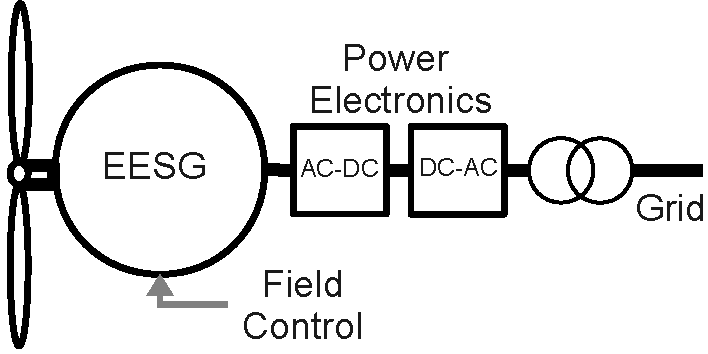
\includegraphics[width=0.5\textwidth]{EESG}
    \caption{Direct drive electrically excited synchronous generator.} 
    \label{eesg}
  \end{figure}

Direct-drive electrically excited synchronous generators are similar to conventional synchronous generators with high number of poles to compensate for the low rotational speed. The generator has a wound rotor winding which requires slip rings to excite. The reactive power and generator output voltage can be controlled using the field current. The assembly is easier compared to permanent magnet machines as there is no magnetic attraction between rotor and stator. The generator does not use rare-earth permanent magnets, so its cost is lower than PM generators. The disadvantages of the EESGs can be listed as:

\begin{itemize}
	\item Largest and heaviest generator type.
	\item Slip rings require regular maintenance.
	\item Losses in the field winding reduce efficiency.
\end{itemize}


  \begin{figure}
    \centering
    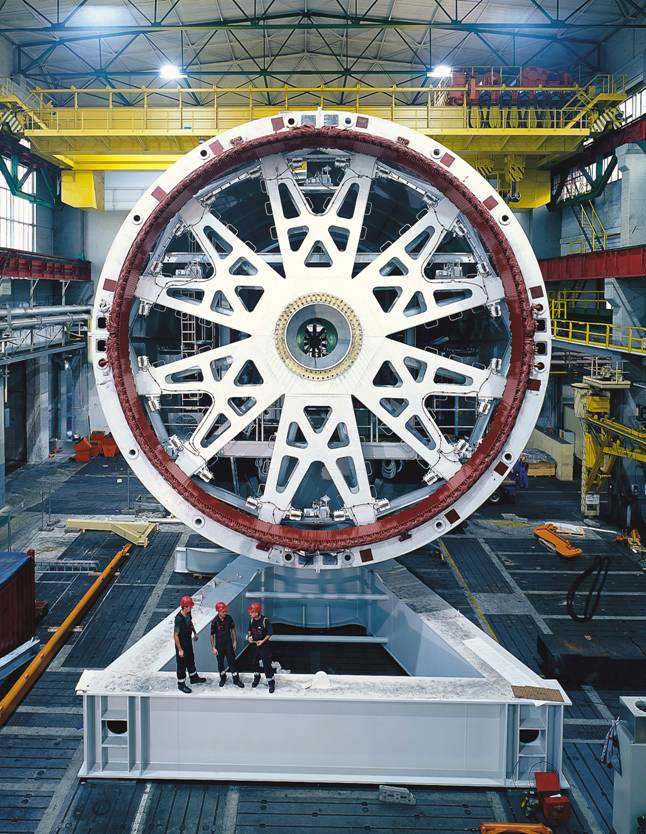
\includegraphics[width=0.5\textwidth]{enercon}
    \caption{Enercon E-126 7.5 MW, 13 rpm direct-drive electrically excited synchronous generator (Courtesy of Enercon).} 
    \label{enercon}
  \end{figure}


\subsection{Permanent Magnet Generators}

Direct-drive permanent magnet generators are synchronous generators that have rare-earth magnets instead of a field winding. They became popular in the recent years due to simple and robust structure. In Figure~\ref{ddpmg}, schematic of a DDPMG is presented. In Figure~\ref{switch}, a 3.8~MW 21~rpm DDPM generator is shown, which is manufactured by the Switch. The generator is mounted directly between nacelle and the blade hubs.

\begin{figure}
    \centering
    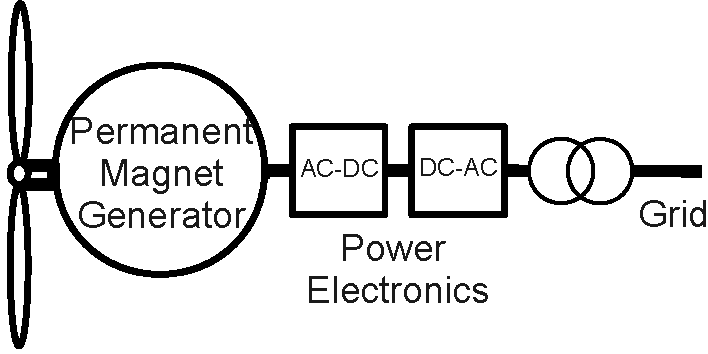
\includegraphics[width=0.5\textwidth]{DDPMG}
    \caption{Direct drive permanent magnet generator.} 
    \label{ddpmg}
\end{figure}


  \begin{figure}
    \centering
    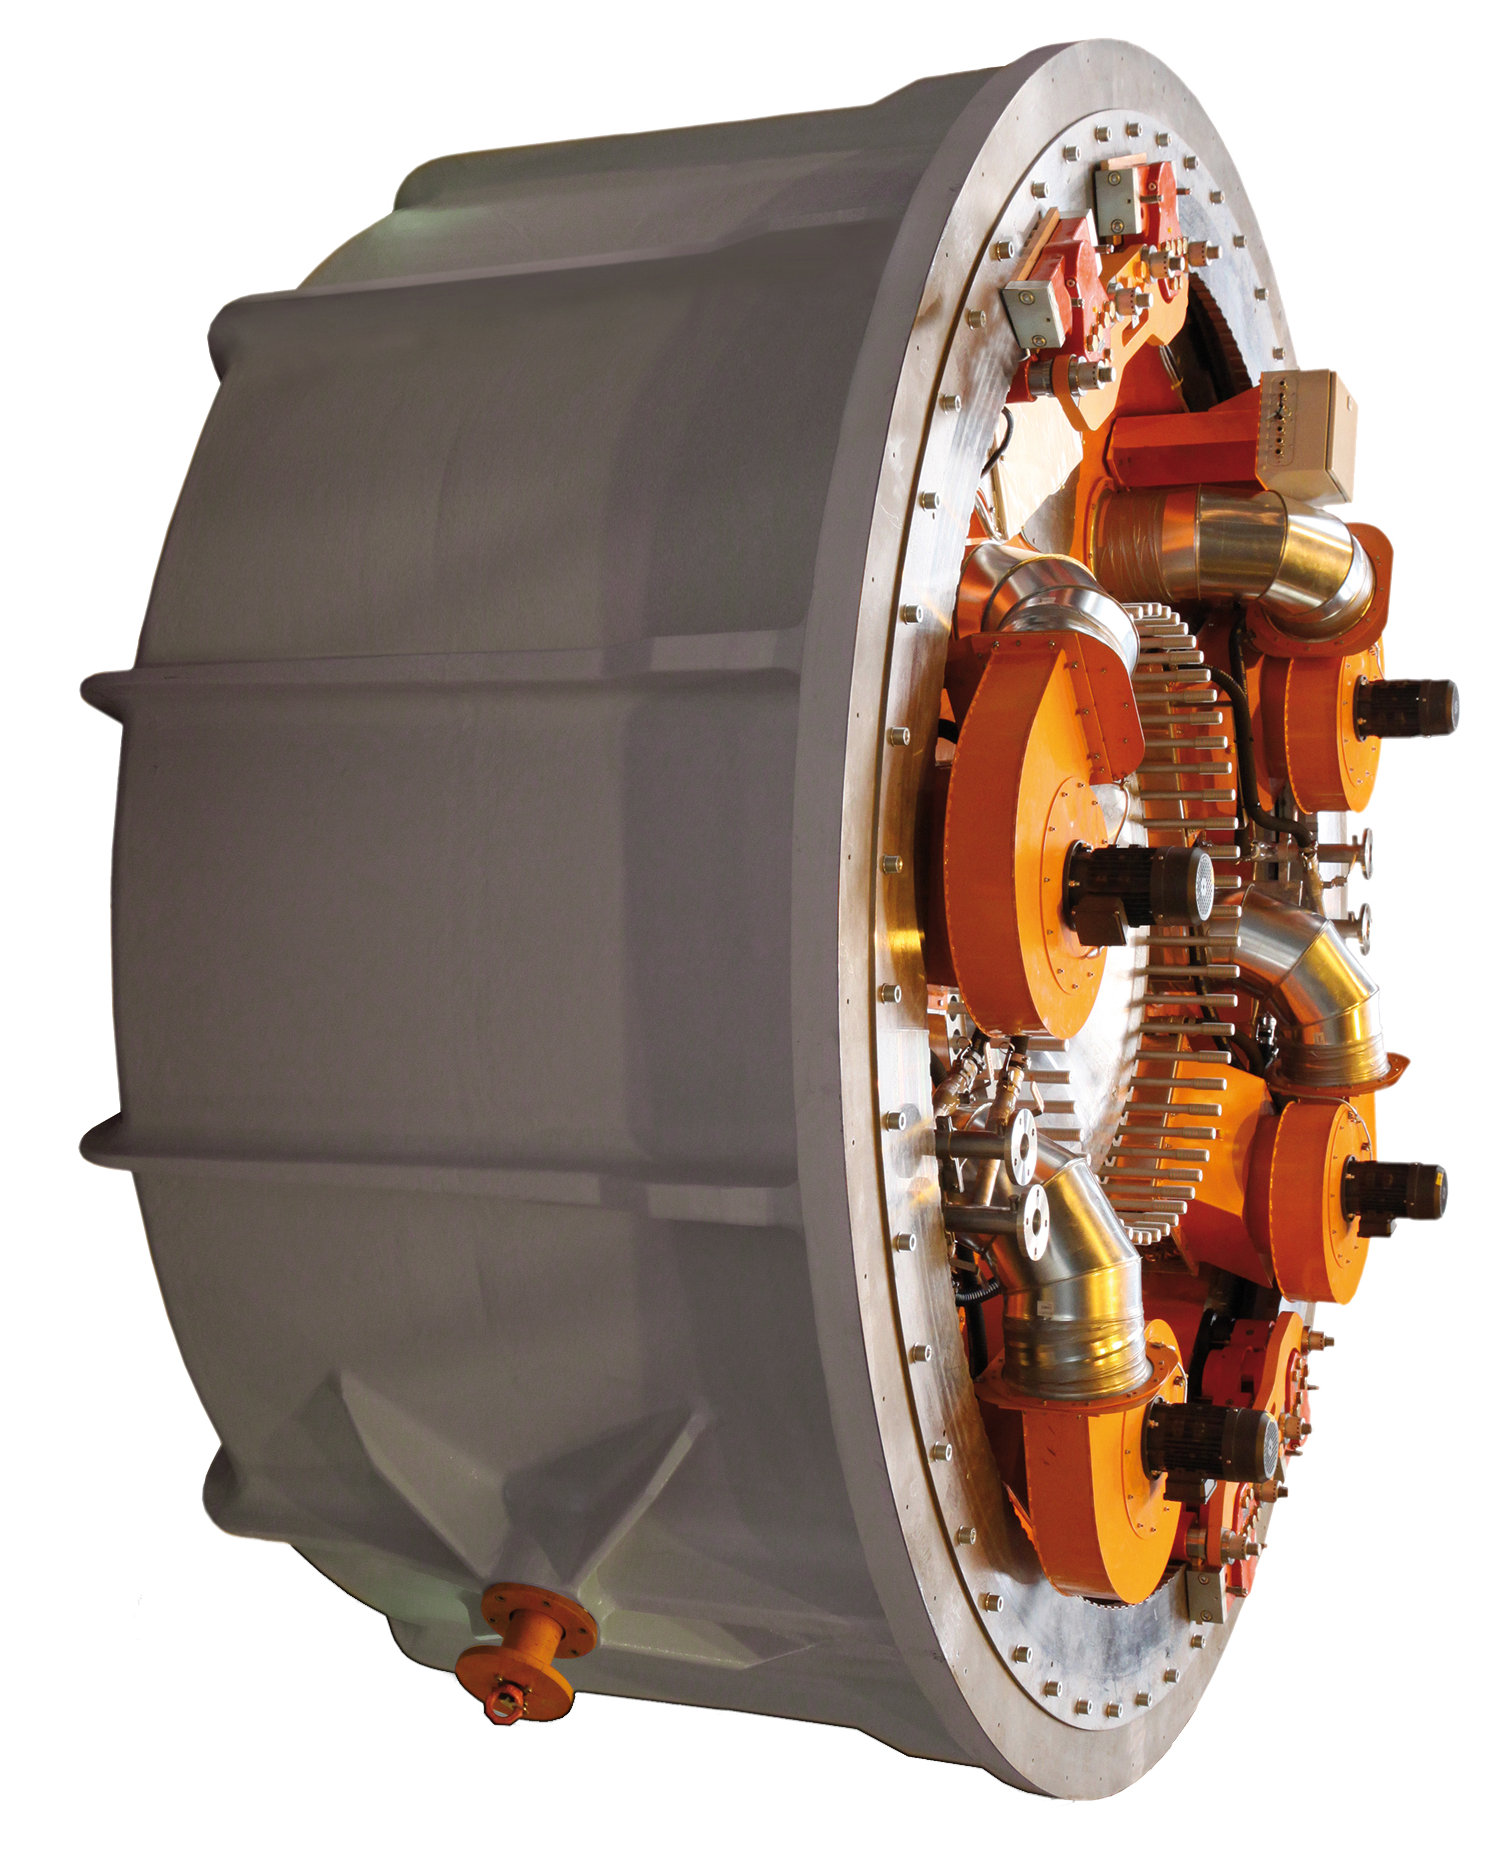
\includegraphics[width=0.35\textwidth]{switch}
    \hfill
    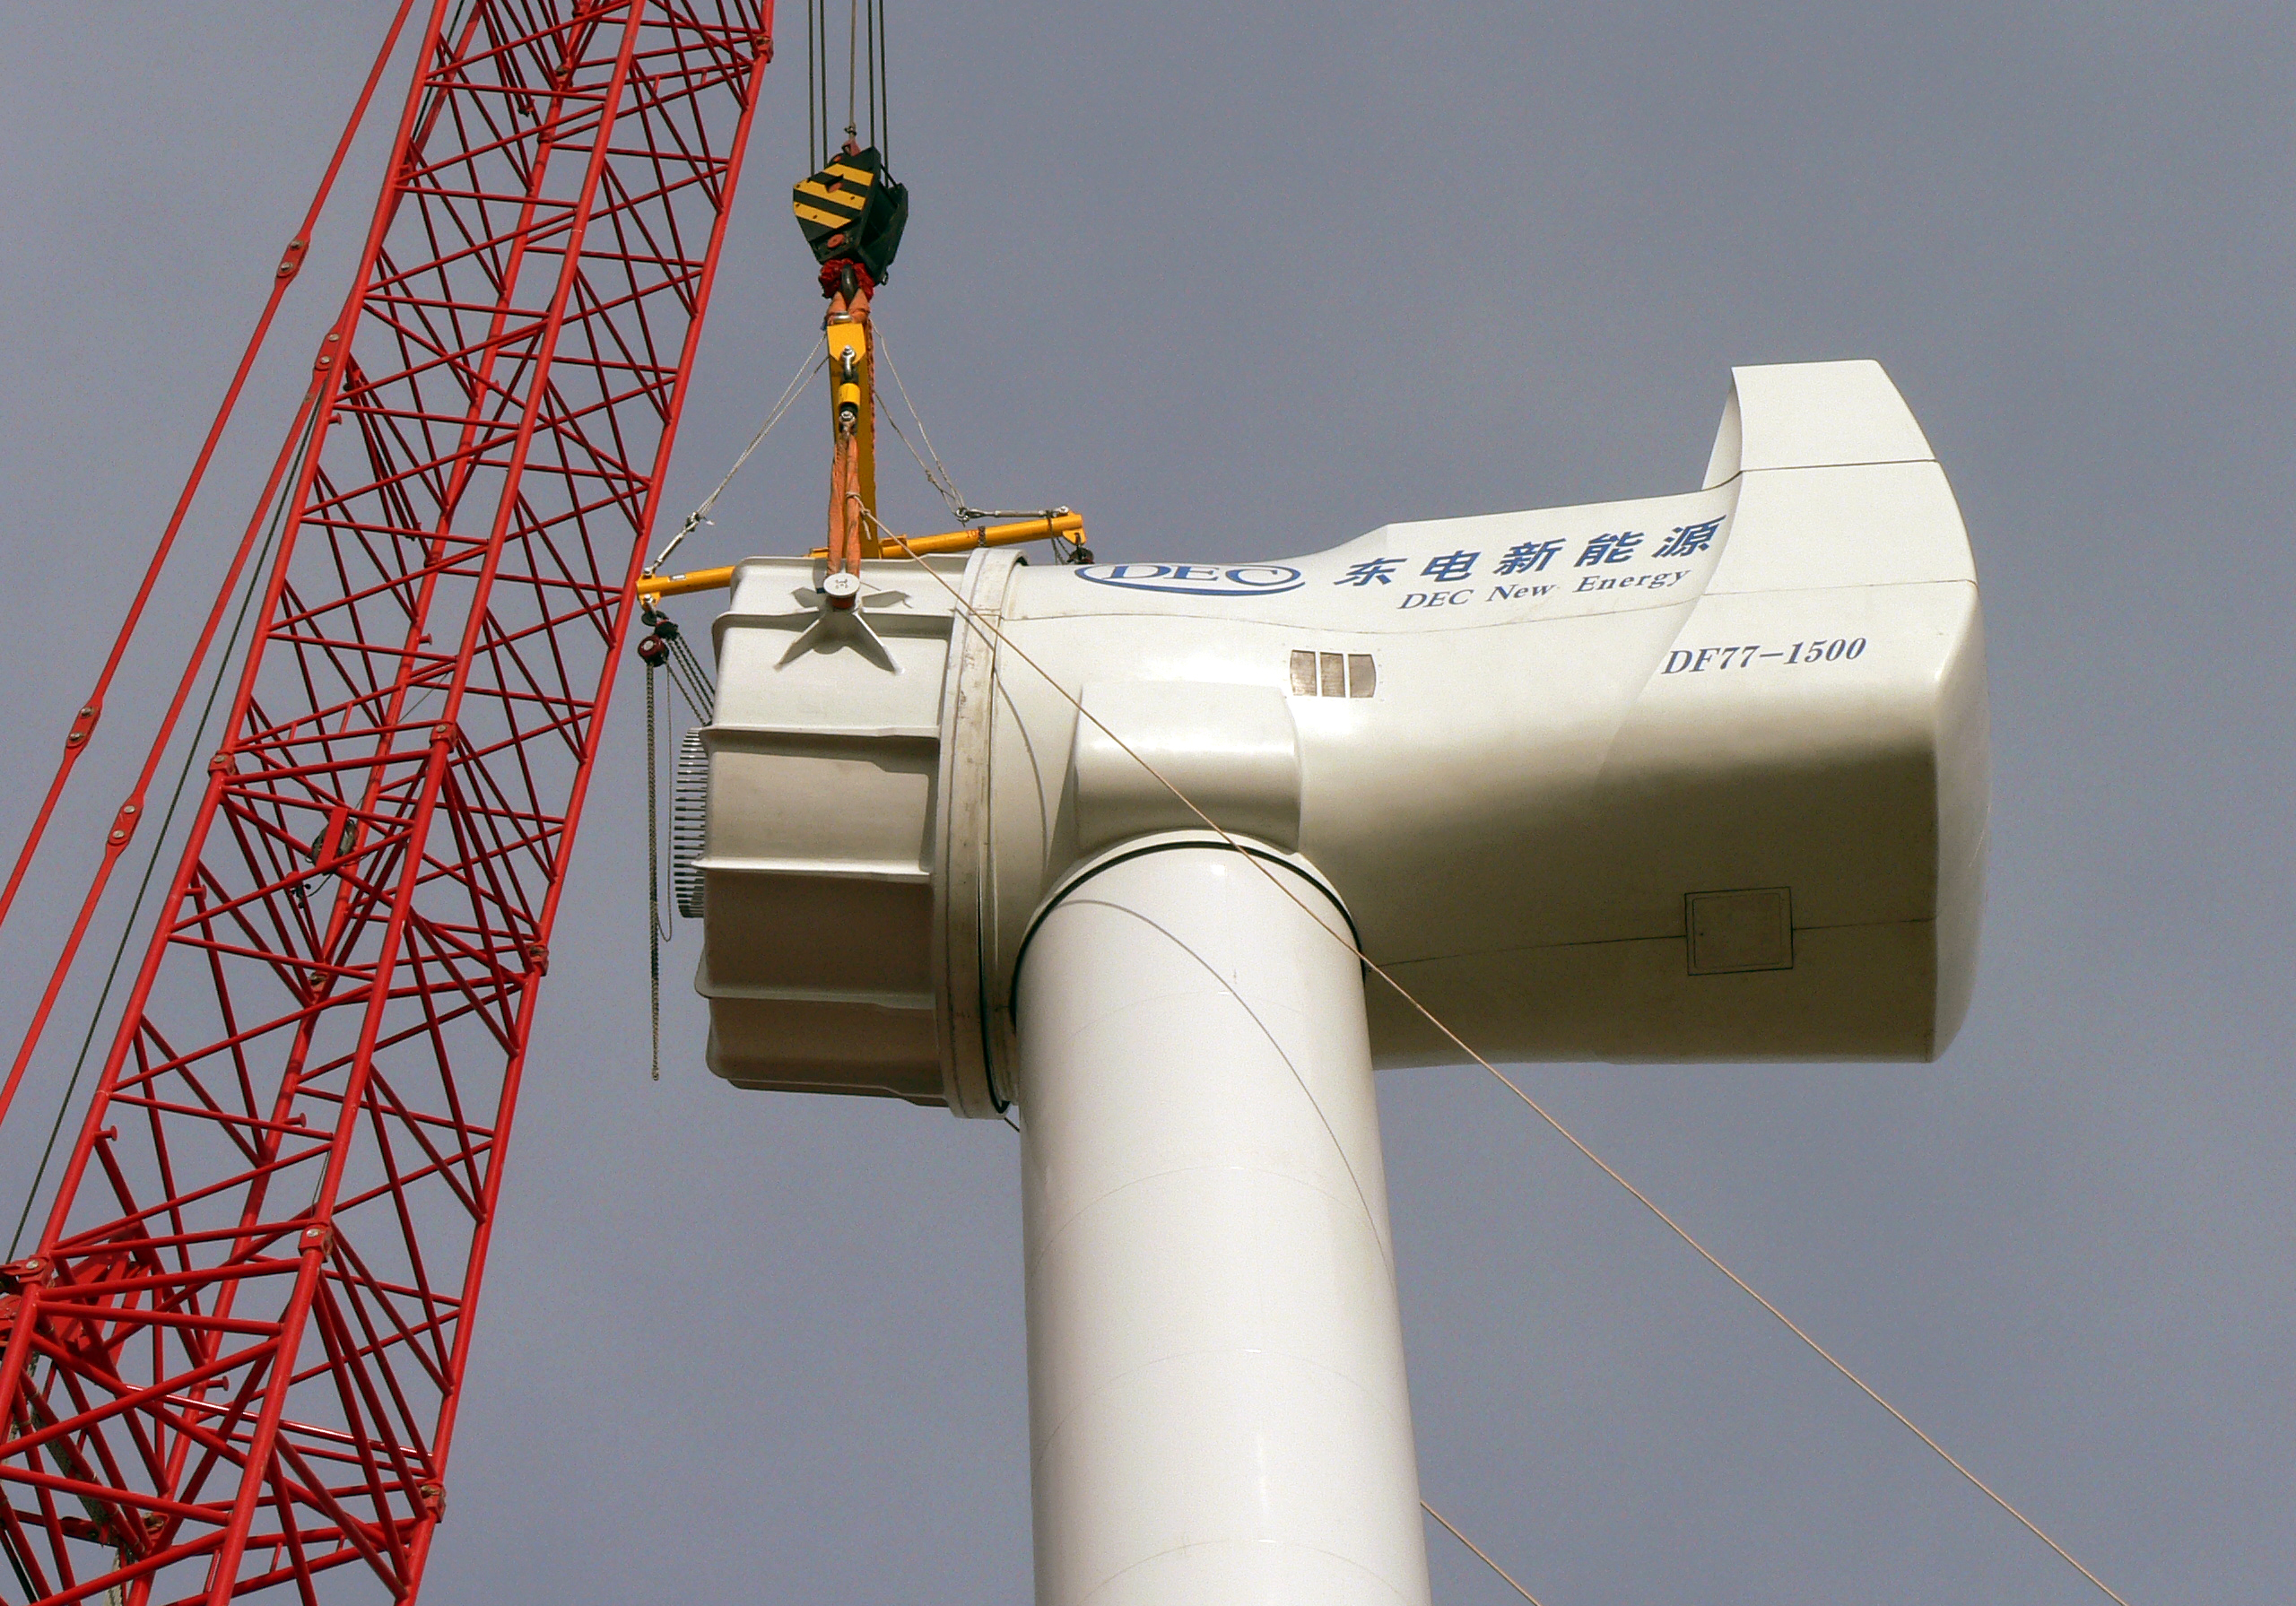
\includegraphics[width=0.6\textwidth]{switch_turbine}
    \caption{3.8 MW, 21 rpm direct-drive permanent magnet generator and installation to the nacelle (Courtesy of The Switch and Dongfang Electrical Machinery).} 
    \label{switch}
  \end{figure}

Compared to geared solutions and electrically excited synchronous generators; direct-drive permanent magnet generators have the following advantages:

\begin{itemize}
	\item The generator has no slip rings, which require regular maintenance.
	\item Having no field winding losses, the generator has a better efficiency.
	\item PM generators usually have higher torque densities.
\end{itemize}

However, the drawbacks of the permanent magnet generators can be listed as:

\begin{itemize}
	\item Iron-cored DDPMGs are difficult to assembly due to attraction force between rotor and stator.
	\item Increased cost due to high price of rare-earth permanent magnets.
	\item Risk of demagnetization of magnets during short-circuit faults.
	\item No control over the induced voltage magnitude.
\end{itemize}

The biggest drawback of permanent magnet generators is the high cost of rare-earth magnets, which has increased more than tenfold between 2009 and 2011 due to export and mining regulations introduced by China  \cite{rareearthelements}. In Figure \ref{neodymium_price}, the price variation of Neodymium Oxide is presented. Although the prices of permanent magnets came down after the peak in 2011, they are still volatile and still four times more expensive compared to five years ago. It is stated in \cite{Moss2011} that the future DDPMGs are in risk due to high demand of rare-earth metals  and supply chain problems due to political risk.  

\begin{figure}[]
\centering
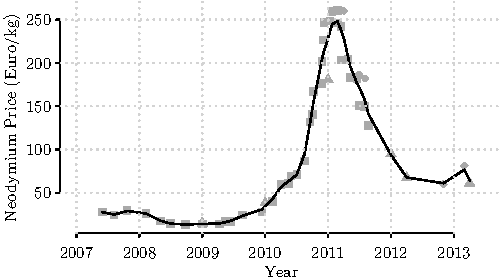
\includegraphics[]{neodymium_price}
\caption{Neodymium Oxide price variation between 2007 and 2013 (data points obtained from Peak Resources Ltd and Lynas Corp.).}
\label{neodymium_price}
\end{figure}

There are a few permanent magnet topologies that aim to achieve higher torque densities. One of the best candidates is the transverse flux permanent magnet (TFPM) machine. In a TFPM machine the winding space can be increased without decreasing the available space for the main flux \cite{Bang2010}. Thus, the machine can have a short pole pitch which helps to increase the frequency and magnitude of the induced voltage at low rotational speeds. In \cite{Bang2010}, different TFPM machine topologies are summarised. It is stated that, a 5~MW TFPM machine is  25\% lighter than a conventional PMG. In general, TFPM machines have simple windings and higher torque densities. On the other side, the flux path is more complex making the mechanical design and manufacturing more complicated \cite{Bang2008,Bang2009}.

\section{Hydraulic Power Take-off Systems}

Hydraulic transmission systems are proposed to drive the generator at synchronous speed (i.e. 1500~rpm for a 4-pole machine connected to 50 Hz grid) regardless of the wind turbine speed. Thus, the generator can be directly connected to the grid eliminating any power electronics. There are two main concepts as presented in Figure~\ref{hydraulics}. In the first configuration, a gearbox is used to couple the hydraulic transmission system, where in the second configuration, there is no mechanical gearbox and the hydraulic pump is directly coupled to the turbine. The output speed of the hydraulic transmission is controlled to keep the generator speed constant.

  \begin{figure}
    \centering
    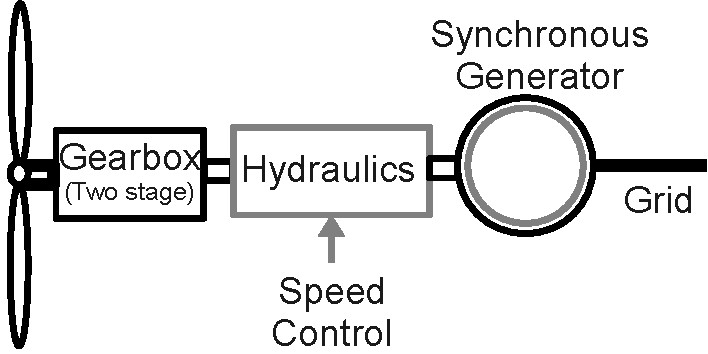
\includegraphics[width=0.45\textwidth]{hydraulics}
    \hfill
    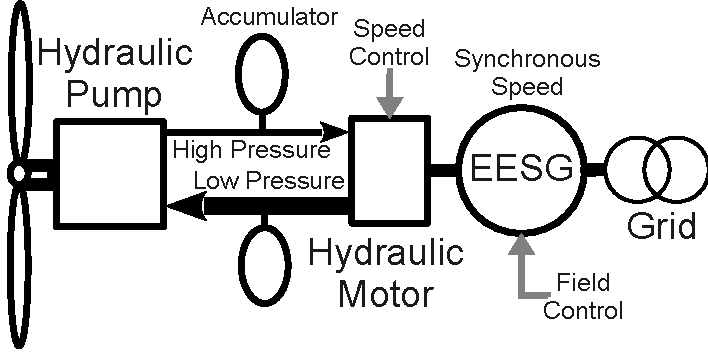
\includegraphics[width=0.45\textwidth]{EESG_hydraulics}
    \caption{Hydraulic system coupled with two-stage gearbox and synchronous generator and power take-off system with hydraulic transmission and synchronous generator } 
    \label{hydraulics}
  \end{figure}

Voith Turbo designed a 2~MW wind turbine hydraulic transmission system, which is presented in Figure \ref{voith}. A conventional synchronous generator is directly connected to the medium-voltage grid without intermediate electrical stages such as power electronics and step-up transformer. The absence of power electronics and transformer means reduced cost and increased reliability.

  \begin{figure}
    \centering
    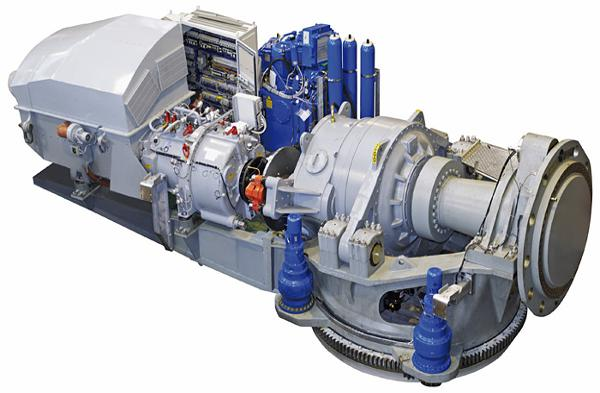
\includegraphics[height=1.2in]{voith_windrive}
    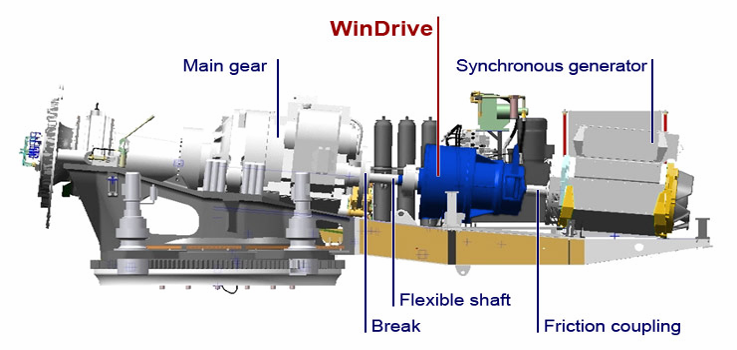
\includegraphics[height=1.2in]{voith_schematic}
    \caption{Windrive 2~MW power take-off system with hydraulic transmission (Courtesy of Voith Turbo).} 
    \label{voith}
  \end{figure}

Artemis Intelligent Power designed a digital controlled hydraulic transmission system, which ensures fast response and efficient operation. Artemis Intelligent Power is designing a 7~MW hydraulic power take-off system, which has a digital displacement pump that drives two independent hydraulic motors and two synchronous generators. Double generator configuration introduces redundancy in the system. Thus, even if one of the generators fails the other one can continue to operate until the next maintenance. Furthermore, at partial loads one of the sets can be idled to increase the overall efficiency.

The weak point of a hydraulic system is the fault ride through capabilities. Since there are no intermediate stages between generator and grid, in case of a grid-fault the control loop of the hydraulic system should be fast enough to respond within grid requirements. Although, mechanical control systems may not be fast enough, Artemis Intelligent Power's electronically controlled hydraulic valves decrease the reaction time of the system. In \cite{artemis}, it is claimed that a control bandwidth up to 20~Hz is achievable.

\section{Generators with Single Stage Gearbox}

Direct-drive generators have many advantages compared to geared generators. The most obvious one is the higher availability and reduced maintenance costs. However, direct drive generators are large and heavy. The middle road between direct drive generators and high speed generators is a hybrid solution with a single-stage planetary gearbox and a medium-speed generator \cite{Li2009}. The generator can be a permanent magnet generator or a doubly fed induction generator. A medium-speed generator reduces the cost compared to a direct-drive generator. Moreover, the high-speed stage of the gearbox, which is considered to be the least reliable section, is eliminated. 

The idea was first introduced by Multibrid of Germany. This concept has gained much attention because it has lower generator cost than the direct-drive concept, and the lower-gear box cost, higher availability and operating reliability than the multiple-stage geared drive concept. In summary, the advantages of the single stage gearbox concept are;

\begin{itemize}
	\item Reasonable overall reliability. The low-speed gear stage is more reliable than multiple-stage gearboxes.
	\item Decreased generator mass and cost compared to direct-drive systems.
	\item Higher utilization of magnetic materials with increased rotational speed.
\end{itemize}

Thus, by accepting a small risk on the gearbox side high mass and cost of direct-drive systems can be mitigated \cite{Bohmeke2003}. Areva Multibrid 5~MW  turbine (see Figure \ref{multibrid}) has an integrated gearbox and generator design. The turbine has a single main bearing and has no main shaft. By this way, the nacelle mass is reduced and possible bearing problems are minimized. 

  \begin{figure}
    \centering
    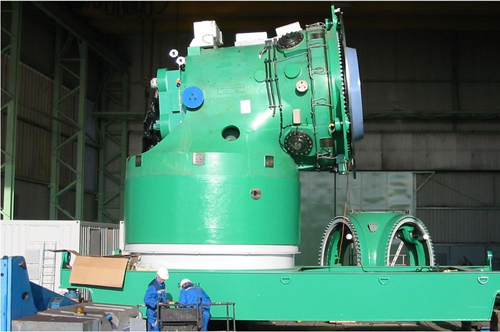
\includegraphics[width=0.5\textwidth]{multibrid}
    \caption{Areva 5 MW Multibrid wind tutbine with combined gearbox and geratator (Courtesy of Areva).} 
    \label{multibrid}
  \end{figure}

\section{Comparison of Generators}

!! Bi yerlere yedir

The different drive-train options have been compared in the previous section. The advantages and disadvantages of these power take-off systems have been tabulated in Table~\ref{generator_comparison}.

\begin{table}[t]
  \centering
  \begin{tabular}{l|cc|cc|cc|}
	  &  \multicolumn{2}{|c|}{Multi-Stage Gearbox} &  \multicolumn{2}{|c|}{Single-Stage Gearbox} &  \multicolumn{2}{|c|}{Direct-Drive} \\
	& DFIG & Hydraulics & DFIG & PMG & PMG & EESG \\
	  \hline
	  Mass & \star\star  & \star\star\star & \star\star\star & \star\star\star & \star\star & \star\\
	  Size & \star\star\star & \star\star\star & \star\star\star & \star\star\star & \star & \star \\
	  Efficiency & \star & \star\star & \star\star & \star\star\star & \star\star\star & \star\star\star \\
	  Reliability & \star & \star\star & \star\star& \star\star & \star\star\star & \star\star\star \\
	  Cost & $\star\star$ & $\star\star\star$ & $$\star\star\star$ & $\star\star$ & $\star$ & $\star$ \\
	  \hline
   \end{tabular}
  \caption{Comparison of different power take-off systems.}
  \label{generator_comparison}
\end{table}


%The system cost and mass of different power take-off systems have been compared in UpWind project for turbines with a power rating of 0.75~MW, 3~MW, 10~MW \cite{upwind2011}. The system cost includes, generator active material cost, generator construction, the gearbox (for geared PTO systems), power electronic cost and electrical subsystem cost. The generator system weight is the combined weight of generator (inactive and active materials) and gearbox. The graphs show that direct-drive generators have the highest mass and cost. The lightest solution is the permanent magnet generator connected to a multi-stage gearbox. The least expensive option is given as the doubly-fed induction generator connected to a single stage gearbox.


\section{Novel Generator Systems}

There are also some novel generator concepts that aim to eliminate the problems of the existing topologies such as high tower mass, reliability or regular maintenance requirements. These problems arise especially for turbines larger than 5~MW. Although there are not proved commercial products for these generator types, they may become popular in the following decades as the average size of the offshore wind turbines continue to increase.

\subsection{Ironless Permanent-Magnet Generators}

Electrical steel laminations are used in the stator and rotor core of conventional permanent magnet generators, The electrical steel has a low magnetic reluctance, however, the assembly and repair of an iron cored permanent magnet generator is very difficult due to high magnetic attraction forces between rotor and stator. Furthermore, a heavier support structure is required to keep the airgap clearance constant and non-balanced forces reduce the lifespan of the generator bearings. These forces can be eliminated with an air cored stator winding design \cite{Mueller2009}. The elimination of these forces reduces the structural mass considerably as described in \cite{McDonald2008b}. Also, the machine can be assembled and maintained much easier. 

  \begin{figure}[t]
    \centering
    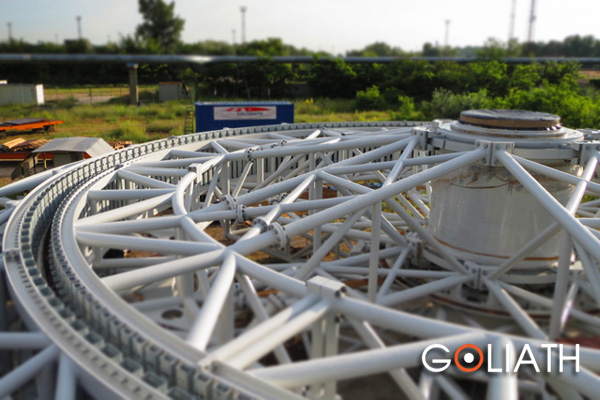
\includegraphics[width=0.5\textwidth]{goliath}
    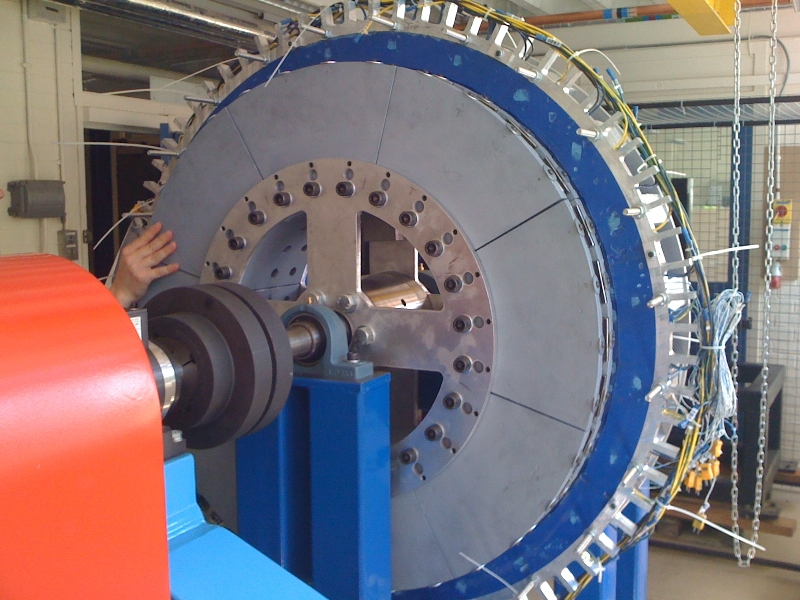
\includegraphics[width=0.45\textwidth]{25kw_cgen}
    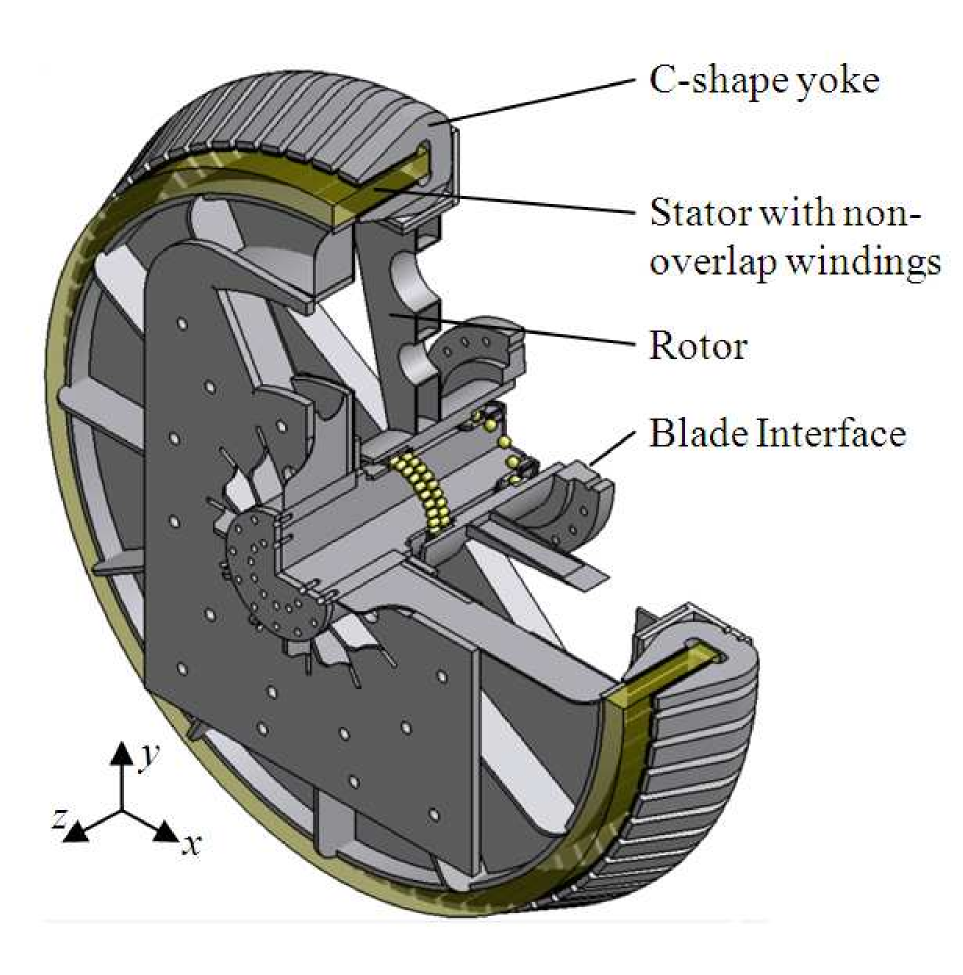
\includegraphics[width=0.5\textwidth]{c-core_kamper}
    \caption{Air cored permanent magnet generators: 3 MW radial flux PM generator (Courtesy of Goliath Wind), 25 kW axial flux PM generator (Courtesy of NGenTec), 300 kW radial flux PM configuration \cite{Wijk2010}.} 
    \label{air_cored}
  \end{figure}

As an additional advantage, several axial flux permanent magnet machines can be stacked in the axial direction. Thus, each machine can operate independently and the faulty section can be disconnected from the rest of the machine. Thus, the machine can operate at partial load until the next maintenance. 

The disadvantages of air cored permanent magnet generators can be listed as;

\begin{itemize}
	\item Increased magnet mass and cost compared to iron cored PMGs.
	\item Lower air-gap flux density.
	\item Heat transfer from coils is reduced. Additional cooling system may be required.
\end{itemize}

Instead of electrical steel laminations, soft magnetic composites (SMCs) can also be used in armature coils. SMCs can be manufactured in complex shapes, giving more freedom and modularity in the machine design. A spin-out company from University of Oxford: YASA (yokeless and segmented armature) motors utilized SMCs in their PM motors, which is presented in Figure~\ref{yasa_motor}. The motor is optimized for high-torque electric car motors and has a forced-oil-cooling system. The motor has a high efficiency and torque density but the performance and total mass of this machine is not clear for large diameter, low-speed applications.


  \begin{figure}[t]
    \centering
    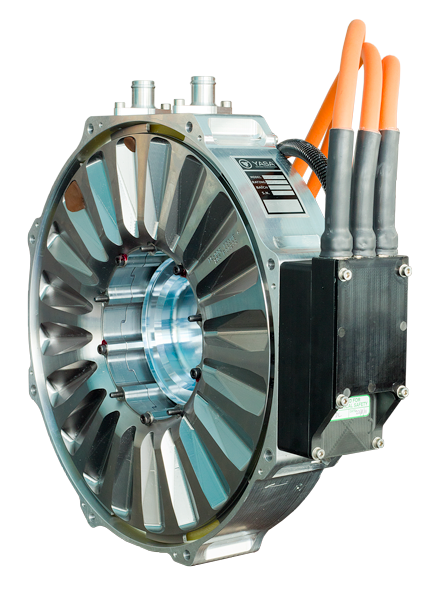
\includegraphics[width=0.4\textwidth]{yasa_motor}
    \caption{YASA (yokeless and segmented armature) motor, 750 Nm (Courtesy of YASA Motors).} 
    \label{yasa_motor}
  \end{figure}

\subsection{Pseudo Direct Drive (Magnetic Gears)}

In pseudo direct drive system, the generator is coupled to prime-mover with an intermediate magnetic transmission. The generator can be integrated with the gearbox as shown in Figure 36. Thus, the input shaft can be connected directly to slow rotating turbine, while actual speed of the generator is maintained at higher values. By this way, the size of the generator can be greatly reduced without using mechanical or hydraulic transmission.

The magnetic gears are contactless, lubricant-free and have no friction. Thus, magnetic transmission offer higher efficiency and reliability compared to geared systems. In a magnetic gear, the generator is not directly coupled with the prime mover; the vibrations are not transferred to the generator side and if input torque exceeds the maximum torque, the magnetic gears just decouple. This is advantageous for some cases, but it also limits the fault-ride-through capabilities of the system.

  \begin{figure}[t]
    \centering
    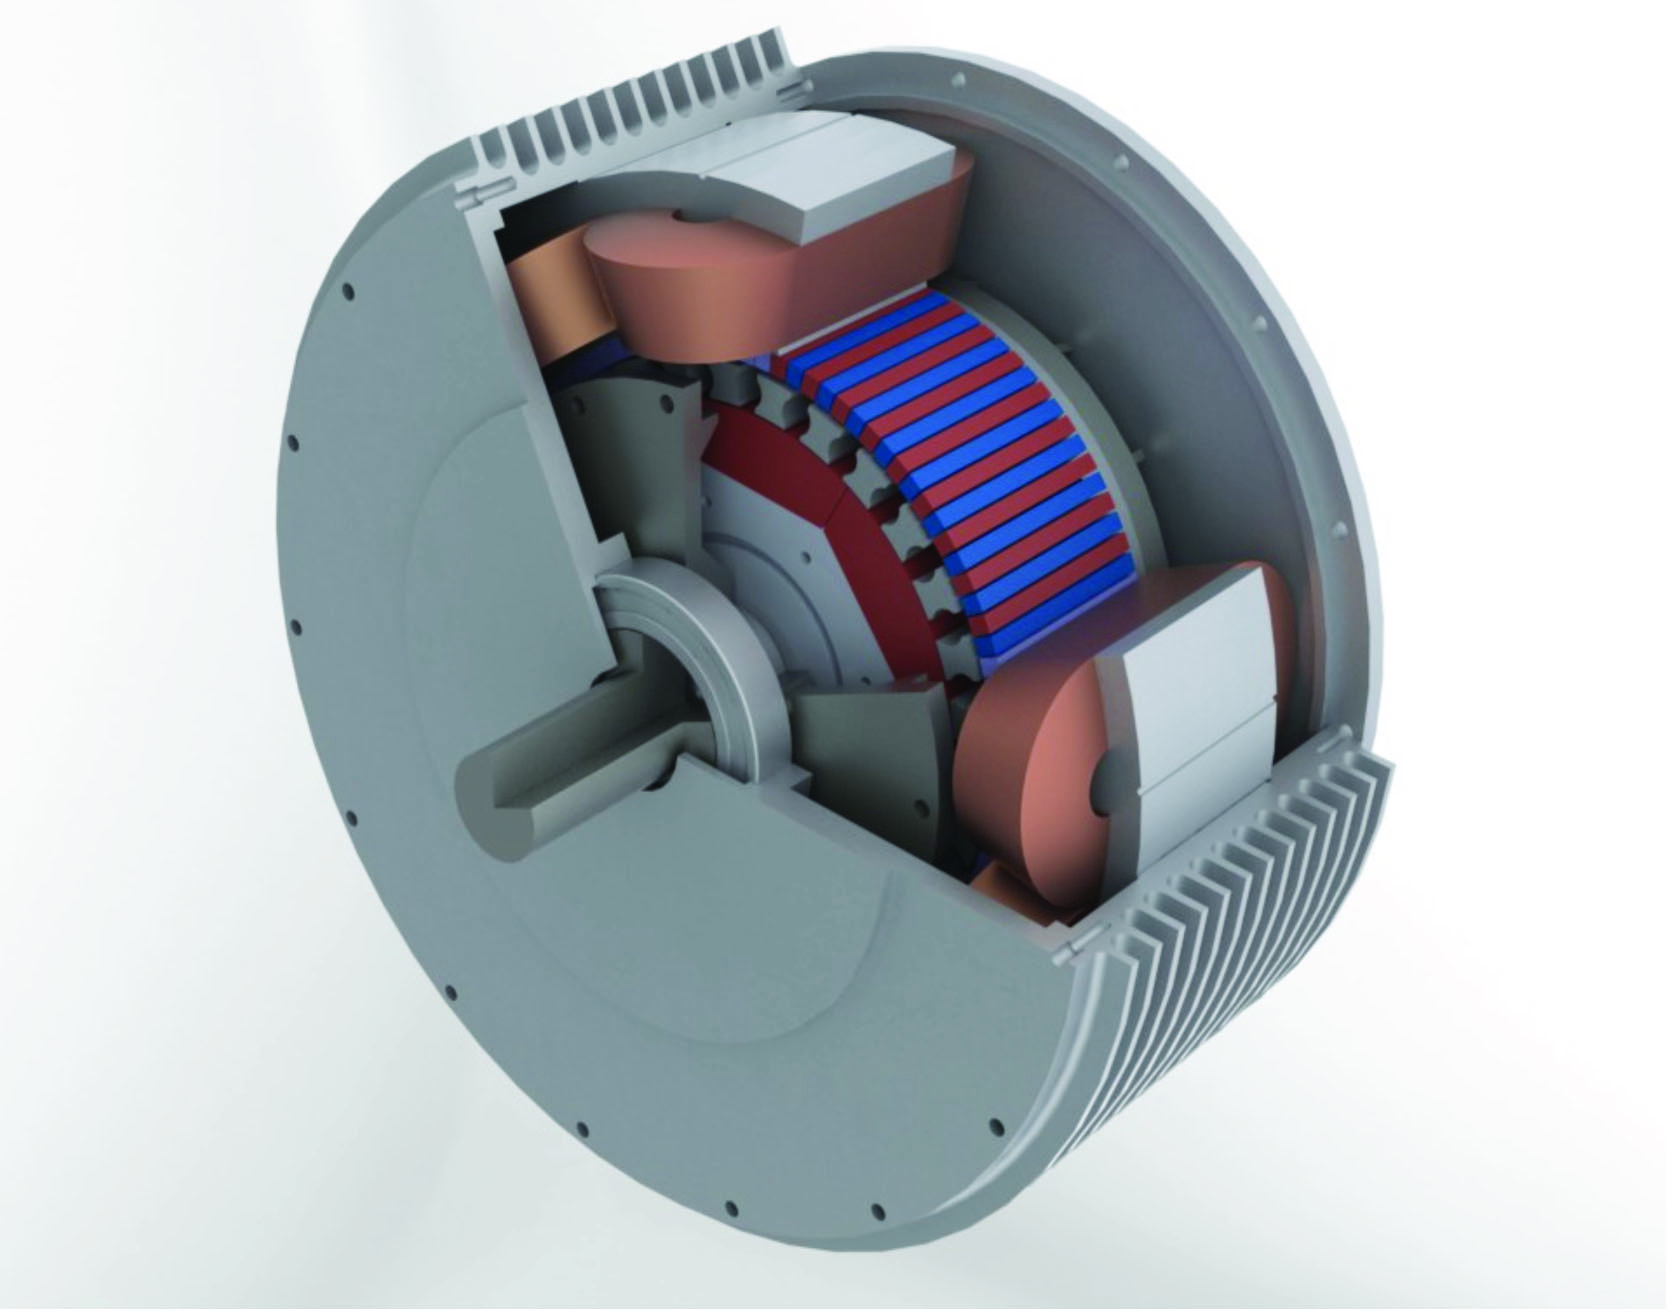
\includegraphics[width=0.4\textwidth]{magnomatics}
    \caption{Combined magnetic gearbox and generators (Courtesy of Magnomatics).} 
    \label{magnomatics}
  \end{figure}


Magnomatics is the leading company in magnetic transmission design. They are developing magnetic gears for electric car motors. Recently, Magnomatics signed a contract with UK Ministry of Defence to develop a magnetically geared propulsion system for ship propulsion. They are also planning to manufacture solutions for renewable energy. 

\subsubsection{Superconducting Generators}

Superconducting electrical machines have drawn interest since the discovery of the first superconductors in 1911, but it was after the discovery of high-temperature superconductors that the research on the applications of superconductivity has been boosted. Superconducting machines have a very high power density and can reduce the size of the machine significantly. For example in Figure \ref{amsc_36mw}, the size and mass comparison between a superconducting machine and conventional motor (ship propulsion motor) is presented.


!! Add size comparison text

  \begin{figure}[t]
    \centering
    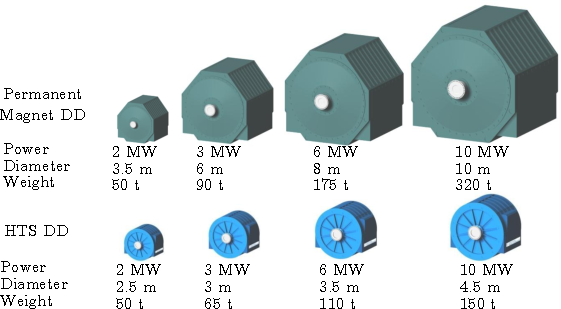
\includegraphics[width=0.8\textwidth]{amsc_ddpm_hts_comparison}
  	\caption{Size and mass comparison of direct-drive permanent magnet generator and superconducting generator for different power ratings \cite{amsc_presentation}.} 
  	\label{ddpm_hts_compare}
  \end{figure}


  \begin{figure}[t]
    \centering
    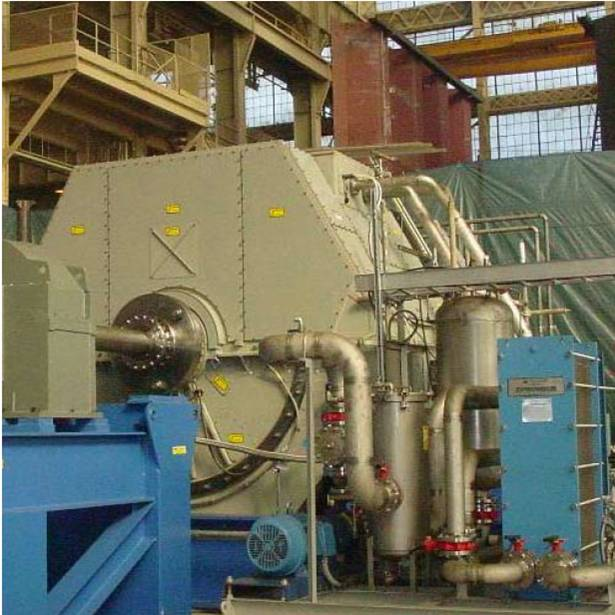
\includegraphics[width=0.45\textwidth]{36MW_AMSC}
    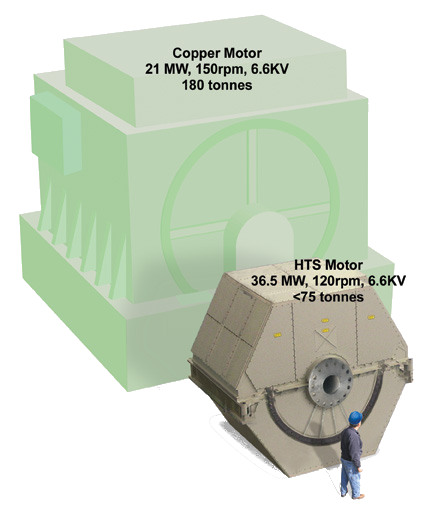
\includegraphics[width=0.4\textwidth]{amsc_36mw_compare}
    \caption{36.5 MW superconducting ship propulsion motor for comparison with a conventional propulsion motor US Navy and size  (Courtesy of AMSC).} 
    \label{amsc_36mw}
  \end{figure}

Some superconducting machine topologies are summarized in \cite{Kalsi2004a,Gieras2008a}. Among these machines, the most common type is a hybrid superconducting synchronous machine which is a synchronous machine with a superconducting dc-field winding. These superconducting machines have high power density but require cryogenic couplers and field excitation brushes in the rotor structure, which causes reliability problems. 

Data from direct-drive systems have been collected to compare mass to torque ratio of HTS machines with other type of generators. The result is presented in a bubble chart in Figure 38. The data for each generator can be found in \cite{Keysan2011b}. The dashed line represents ratio of generator mass to torque for permanent-magnet machines which is estimated as 25 kg/kNm by Bang et al. in \cite{Bang2008}. The Enercon-E112, which has a high mass to torque ratio (66.6 kg/kNm) is the only copper field synchronous generator in the graph. The continuous line represents the linear trend line estimated using the HTS machines in the graph.). It can be seen from the graph that HTS machines are generally lighter than PM generators for applications with torque requirements larger than 3000 kNm. 

**Figure 38 mass comparison graph

There are some companies interested in superconducting wind turbines, Converteam -now acquired by General Electric- proposed an 8 MW, 12 rpm superconducting generator, which will be 5 m in diameter and approximately 100 tonnes \cite{Lewis2007}. 

AMSC aims to manufacture a 10 MW direct-drive superconducting generator: SeaTitan which is shown in Figure 39. The generator will have an outer diameter of 4.5-5 m and have a mass of 150 tonnes \cite{Snitchler2011}.

**resmi cikar

Recently, Department of Energy (U.S.) awarded \$7.5 million to six companies to help develop next generation wind turbines \cite{dep_energy}. Two of these companies are planning to manufacture direct-drive superconducting generators. GE Global Research (in partnership with Superconductor Technologies Inc.) aims to design a 10 MW direct-drive low- temperature superconducting generator –using MgB2 wires. The generator is planned to have a stationary superconducting field winding to reduce cryogenic-coupler faults. The other company is Advanced Magnet Lab. which plans to design a 10 MW, 10 rpm, fully-superconducting generator which will be 70 tonnes. The ac losses on the armature coils can be minimized using their patented double-helix winding arrangement.

The high efficiency of superconducting machines has been emphasized in the first applications, but efficiency is not solely sufficient. In order to penetrate into the renewable energy market,  superconducting generators have to prove that they are also more reliable than alternative power take-off systems such as DDPM machines and geared induction machines \cite{Abrahamsen2010}. In a HTS machine, the cryogenic system holds the risk of decreasing the overall reliability. In particular, the cryogenic pump and couple are the most critical components. The cryogenic coupler can be eliminated by using a stationary superconducting field, which has many advantages \cite{Gieras2008a}:
\begin{itemize}
	\item No cryogenic coupler, more robust and cheap cooling system
	\item No cryogenic coupler, more robust and cheap cooling system
	\item No brushes or complex excitation systems
	\item No centrifugal forces and transient torques that can damage the superconducting material
\end{itemize}


A novel superconducting generator topology has been proposed in \cite{Keysan2011e}. A single loop-shaped stationary superconducting field winding is used in the generator. The rotating parts only consist of modular iron cores. 

**duzenle

\subsection{Generation at Sea Level}

**Hydraulics kismiyla birlestirilebilir

Lower tower top mass is favourable in larger offshore wind turbines, especially for floating platforms. Several hundred tons of nacelle mass may introduce stability issues and increases the installation cost. The tower top mass can be reduced by placing the electrical generator at sea level. This also means easier access to some critical components. The response time of the hydraulic pump and hydraulic motor should be fast enough to satisfy the fault-ride-through requirements of the grid.

ChapDrive is developing a 5 MW hydraulic power take-off system for offshore wind turbines. The project is partly funded by Statoil. Note the hydraulic motor and the generator is placed at ground level, inside of the tower. Top mass of the turbine is expected to be less than 200 tonnes.

University of Delft, applies the same hydraulic system in a slightly different in the We-at-Sea project \cite{Diepeveen2004}. Instead of using individual generators for each turbine, they propose to use a central generator(see Figure \ref{we-at-sea}) unit for all the turbines in the farm. Sea water can be used to transfer energy from turbines to central generation unit. This unit can be placed on shore for near off-shore wind turbines.

  \begin{figure}[t]
    \centering
    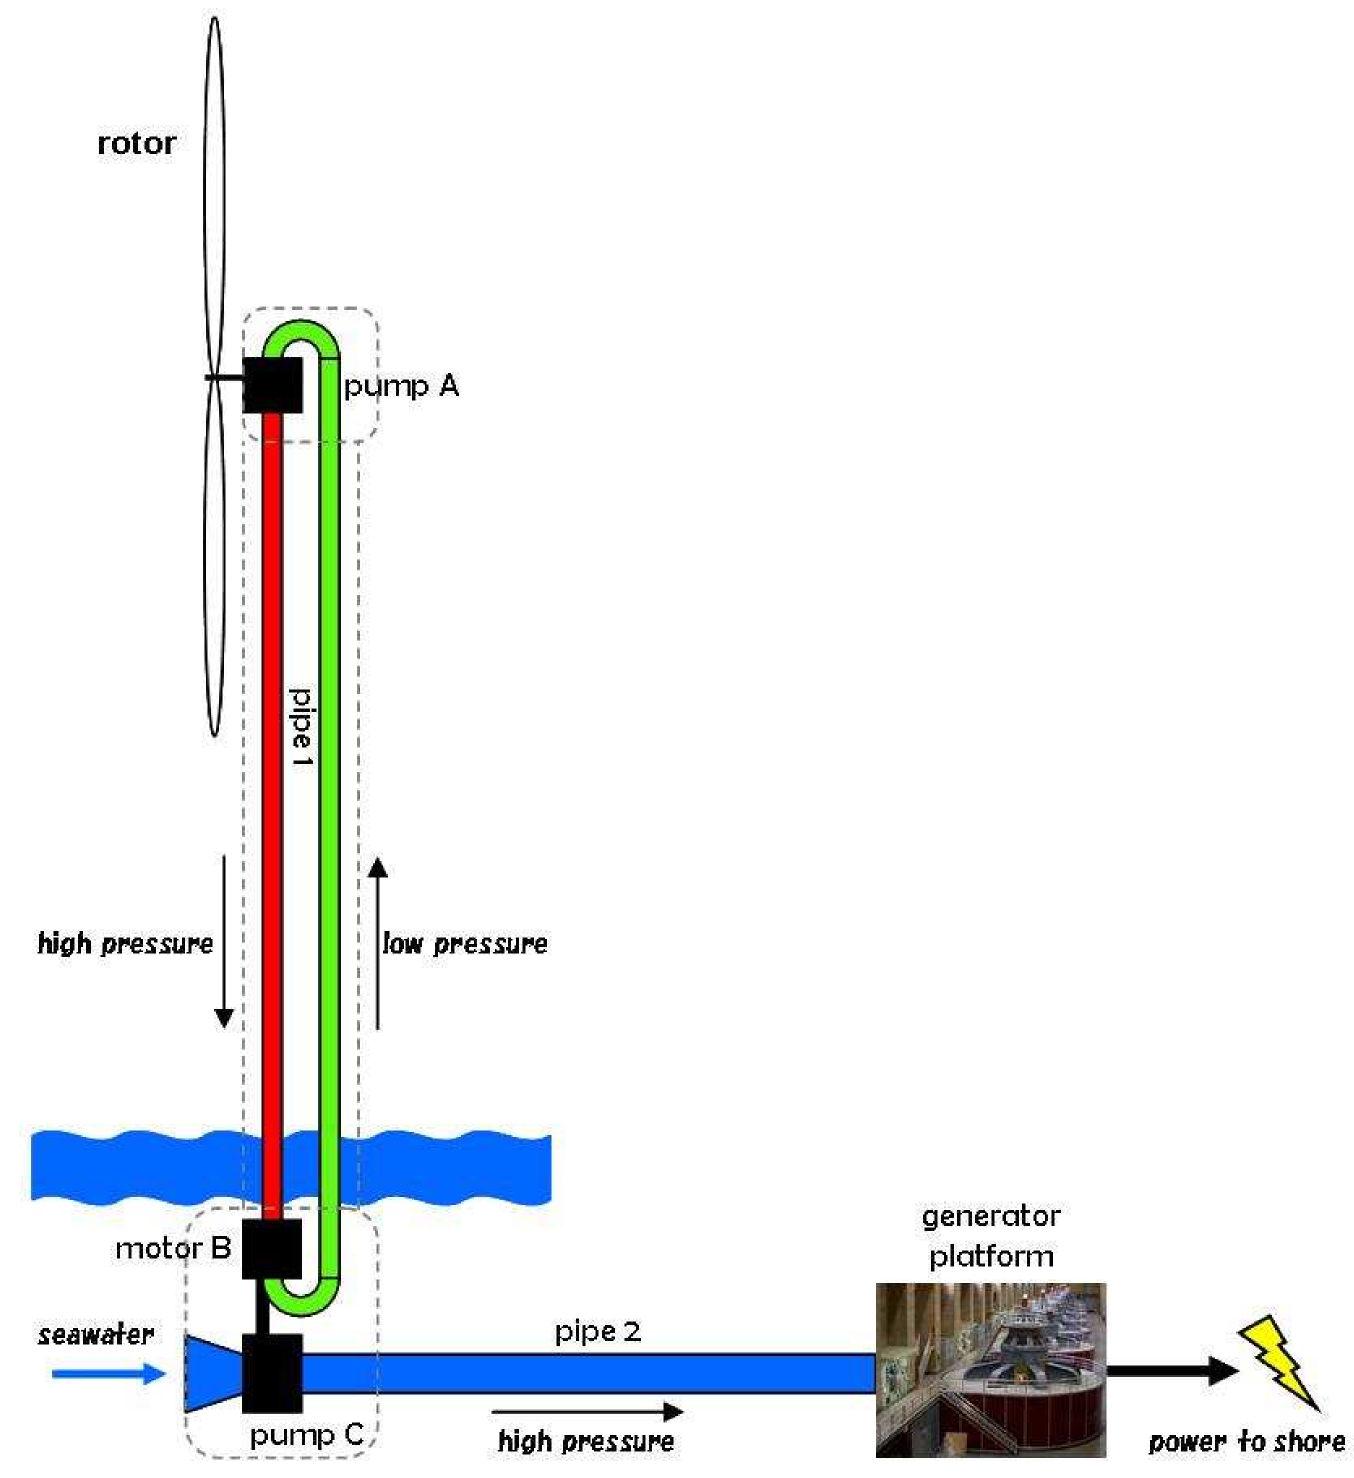
\includegraphics[width=0.45\textwidth]{we-at-sea}
    \caption{Schematic of the seawater-based hydraulic power take-off system  \cite{Diepeveen2004}.} 
    \label{we-at-sea}
  \end{figure}


%----------------------------------------------------------------------------------------
%	BIBLIOGRAPHY
%----------------------------------------------------------------------------------------

\bibliographystyle{unsrt}

\bibliography{../refler/offshore-wind-generators}

%----------------------------------------------------------------------------------------

\end{document}